\section{Task 1: Understanding HSRN researchers' needs and behaviors}

\begin{figure}[t]
    \centering
    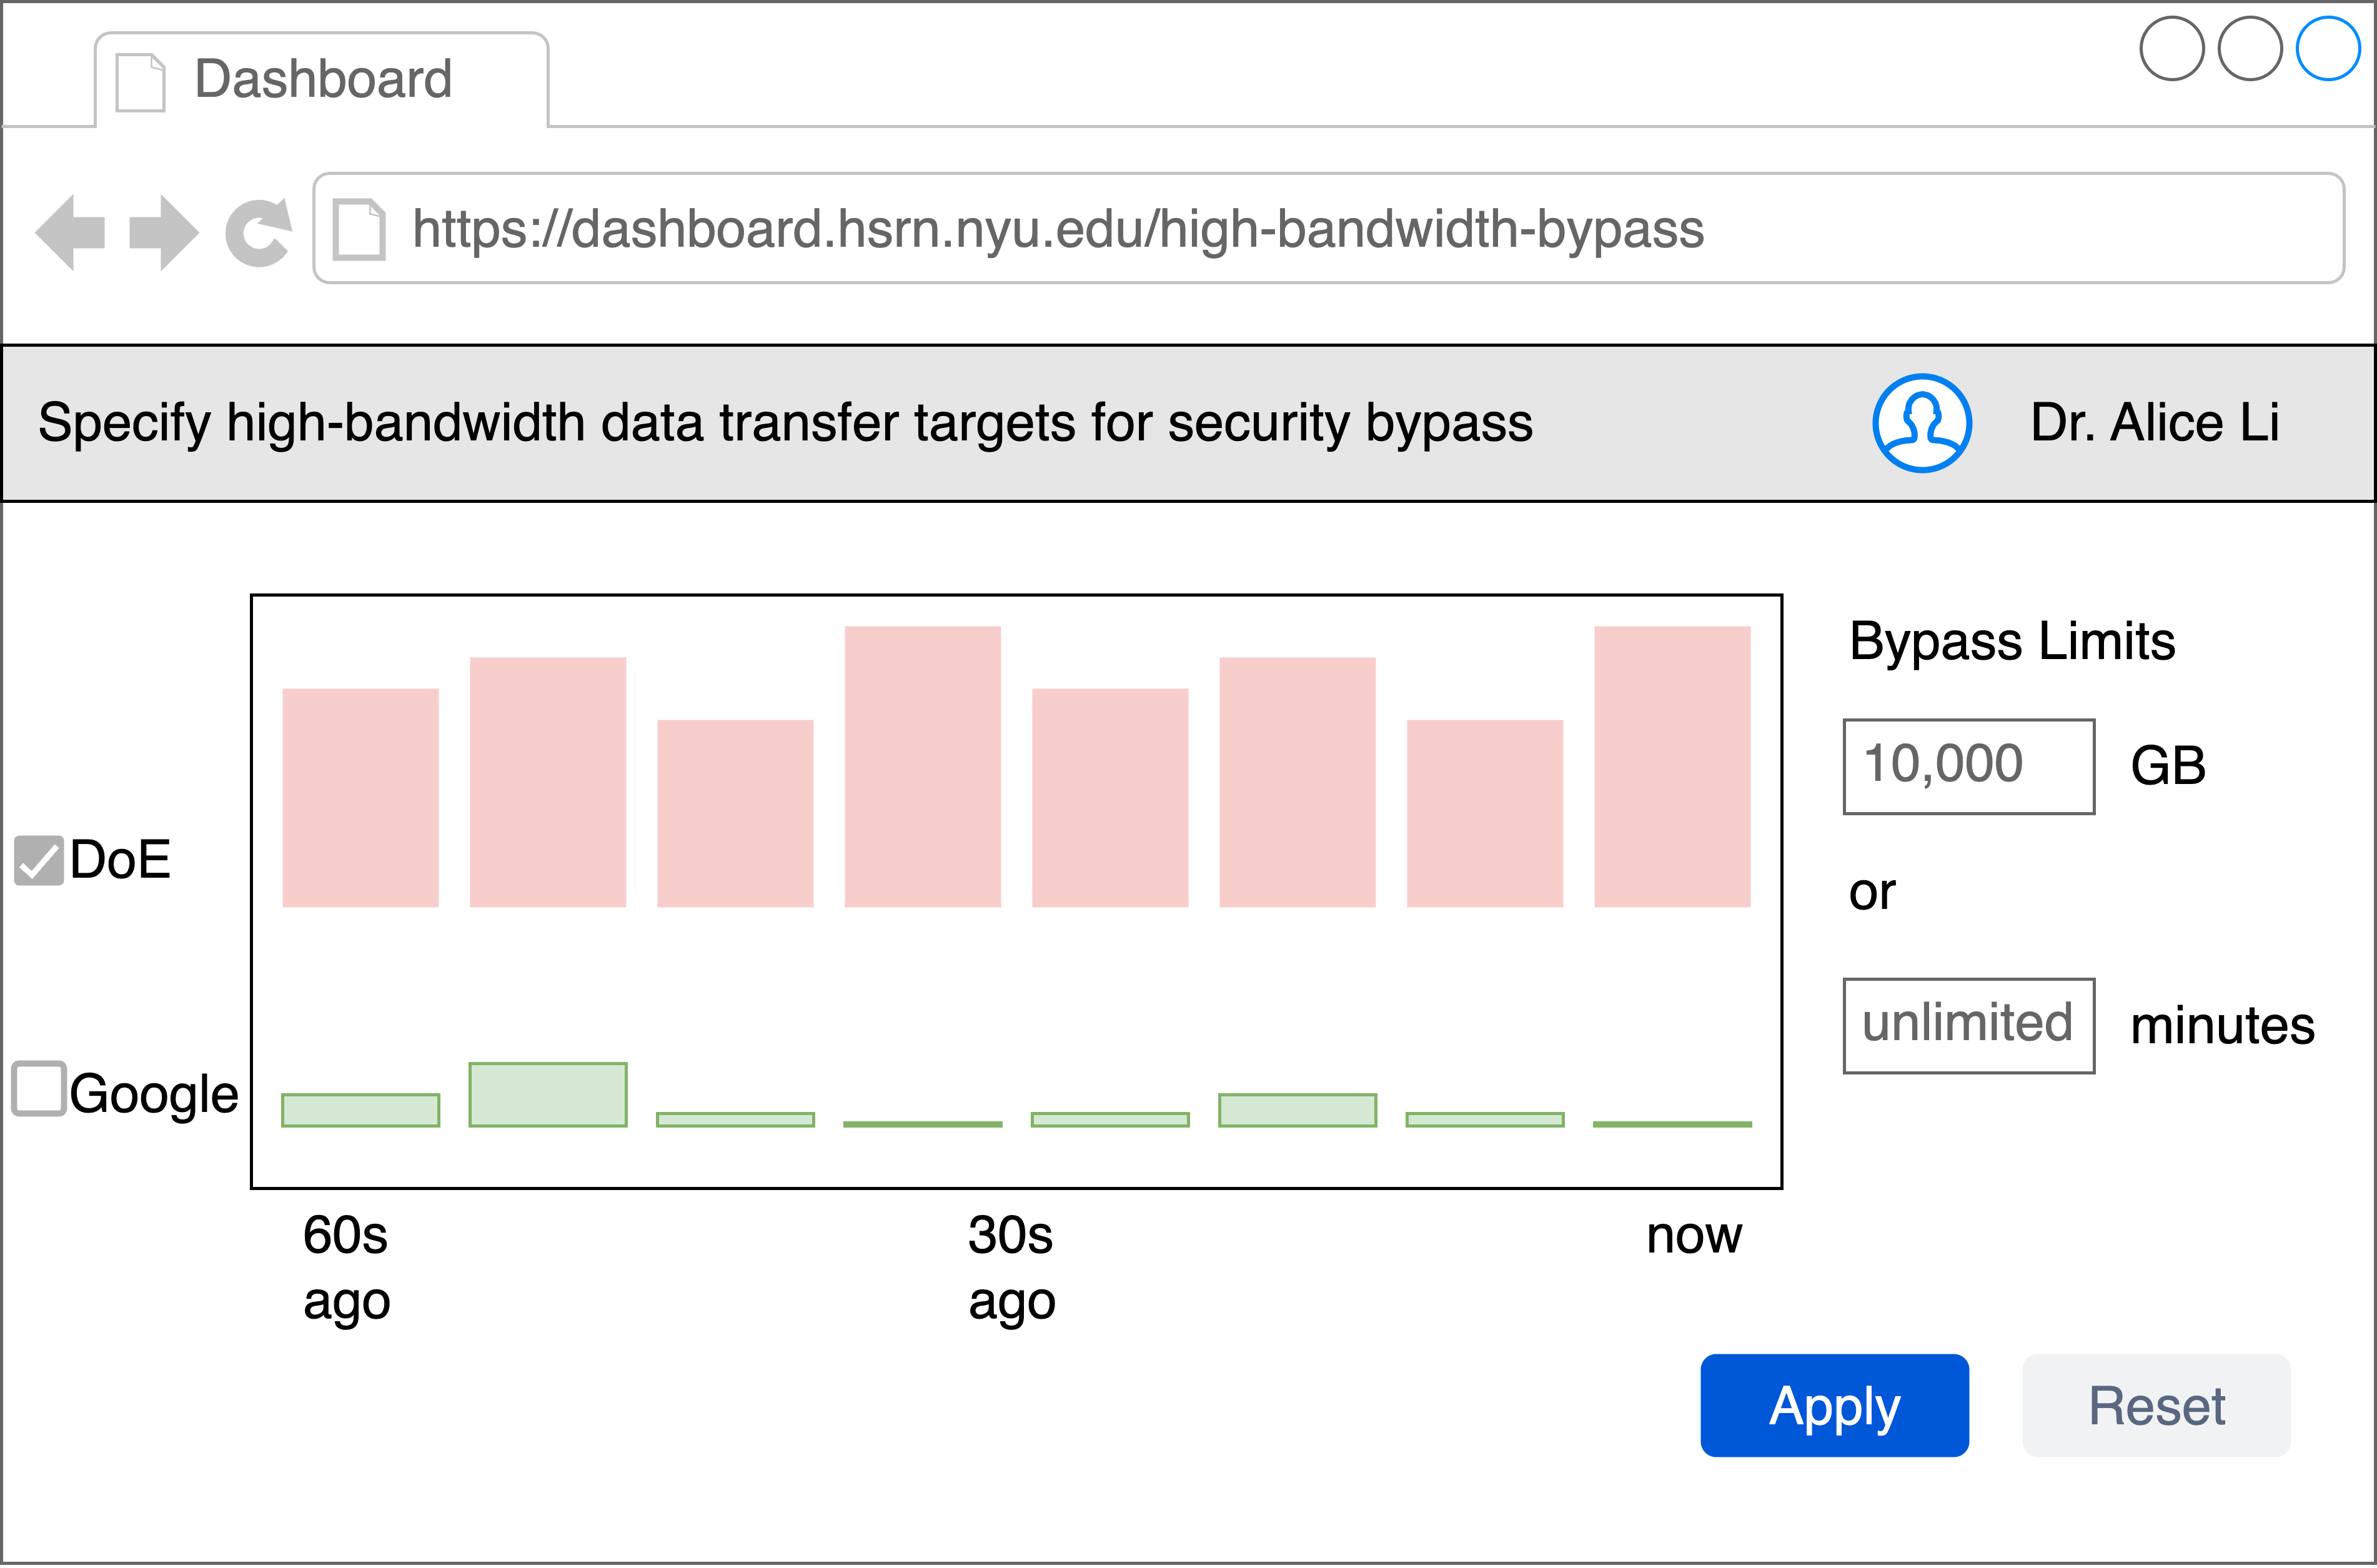
\includegraphics[width=0.7\linewidth]{figures/dashboard.png}
    \caption{A mockup of a part of the dashboard's user interface. Here, a hypothetical physicist, Dr. Alice Li, is shown two network flows and their bandwidth usage from her server, currently connected to the high-speed research network. Only the flows to/from the Department of Energy (DoE) is research related; the Google flows are associated with everyday web traffic. By selecting the DoE flows, the researcher creates an entry in her allow list for DoE. The DoE flows will bypass security checks and go through the fast path [F] (Figure~\ref{fig:system}), until 10,000 GB has been sent.}
    \label{fig:dashboard}
\end{figure}

Before we implement the system, we first need to understand the needs of researchers as reported by researchers, e.g., how they interact with the current HSRN, how they currently request security bypasses with the network administrators, what are their concerns, and what they would like to see as a solution. This human-centered understanding will help us design the user interface and user experience (UI/UX). We will provide the details in Task 1a.

In addition, we will also need to understand the researchers' behaviors as reported by the network traffic, e.g., their network activities and traffic patterns, by conducting passive network measurements. This analysis will facilitate the automatic annotation of the network traffic of users, e.g., which remote destinations the users are contacting and the estimated bandwidth and latency requirements. Such annotations will help us create the initial allow list, annotate the existing workflow, and help researchers make informed decisions when requesting security bypasses in the UI/UX. We will provide the details in Task 1b.

\subsection{Task 1a: Understanding researchers' needs through user studies}

\paragraph{Understanding existing concerns}
Currently, users on NYU's HSRN would go through a manual approval process to request a temporary bypass for their scientific network traffic, such as sending large datasets or initiating low-latency experiments, e.g., AR/VR. Such requests are often highly technical in nature, including such parameters as the wall ports, remote IP addresses, remote ports, and protocols (TCP/UDP), which, accordingly our preliminary experience with users, could be frustrating for many researchers who do not have the necessary technical background. Furthermore, based on preliminary interviews with network administrators at NYU Research Technologies (where co-PI Pahle is a Senior Research Scientist), this process is also frustrating with network administrators, who often have to manually craft the switch rules based on the researchers' requests. We have also heard of instances where a network administrator had forgotten to disable such a security bypass, thus exposing the researcher to unncessary security risks.

To address these issues, we plan to conduct interviews and focus groups to understand the existing pain points. We will recruit volunteers from within the current users' of NYU HSRN. We will set up 30-minute one-on-one semi-structured interviews with individuals, or 60-minute guided focus groups comprising 3-4 researchers, where we ask them to describe their current experience with NYU's HSRN, e.g., what is their usual scientific workload (such as high-bandwidth transfers versus low-latency experiments), any noticeable degradations in network performance without security bypasses, steps they took to request security bypasses, how often they would need security bypasses, how long before their requests were granted, and how long they would need their security bypass for. Also, we will discuss the details of the requests, including how they described their scientific workload, the bandwidth/latency requirements, the destination party contacted, and particular challenges translating these workloads into bypass requests in a way that can be understood by network administrators. We will tie all these responses to demographics, including what type of researchers they are, from which department, and their level of technical expertise.

This exercise will help us not only understand the needs of researchers but also build a qualitative profile of invididual researchers in terms of their usual scientific workloads: Who from which department tends to send/receive high-bandwidth versus low-latency traffic to particular hosts on the same network or to the Internet, using which switch port and destination ports, over which protocol (TCP/UDP), and typically over how long or how many bytes. This profile will be useful in helping us construct an initial personalized allow list in Task 2.


\paragraph{Co-designing UI/UX}
We plan to conduct co-design sessions to make preliminary designs on the dashboard's UI/UX, making sure that the design is consistent with the researchers' scientific workflows.
Based on our preliminary analysis, typical scientific workloads include two type of network flows: high-bandwidth flows (e.g., for file transfers) and low-latency flows (e.g., for robotics and AR/VR experiments). Here, we use the canonical definition for network flows, which specifies the following five values: the source and destination IP addresses, source and destination ports, and the protocol (TCP/UDP).

From the researcher profile we collected from Task 1a, we will separate the researchers into two groups: one group who self-identifies as conducting mostly high-bandwidth transfer (e.g., physicists sending data to government agencies); and one group who self-identifies as requiring low-latency applications (e.g., roboticists and AR/VR researchers). For each group, we will recruit 3-4 volunteers per co-design session. Within each session, we will ask the participatns to imagine having a self-service portal to specify their workloads and request security bypass---for example, how to describe their workload (e.g., in terms of expected time of completion and number of bytes transffered), how to describe the intended destinations (e.g., in terms of names of government agencies, institutions, IP addresses, or domain names), and how security may play a role in their scientific workloads (e.g., sensitive versus non-sensitive information). During this process, we will guide the participants to sketch out desired user interfaces, how one screen flows to another, and expected actions from each screen.  We will also encourage the participants to design the sketches to integrate into their existing scientific process and avoid impeding their research (unlike the current manual process of requesting security bypasses).

We show an example of a dashboard in Figure~\ref{fig:dashboard} for researchers with high-bandwidth workload. A physicist, for instance, could be regularly transferring large datasets with the Department of Energy (DoE). In one sample use case, the physicist would start the data transfer first, which, by default, goes through the slow path and subject to packet inspection by security appliances. The physicist would now open the dashboard, which lists the bandwidth consumption on his device to various destinations, including DoE and other web traffic (e.g., to Google). We would highlight the DoE transfer because the transfer is already consuming significant bandwidth and also based on user studies the researcher claims their typical workloads include DoE data transfers. This highlight would nudge the researcher toward selecting the DoE network flows for security bypass. Once the physicist clicks the ``Apply'' button, we would expect the system to automatically reroute the ongoing DoE transfer to the fast path (Task 2).


\paragraph{Preliminary work}
We have done some preliminary informal interviews with existing researchers of NYU's HSRN, including roboticists, physicists, AR/VR researchers, and media/arts researchers (whose Letters of Support have been included in this proposal). These informal interviews have revealed much frustration from the researchers in requesting security bypass. Also, we have learned about the two basic types of workloads---i.e., high bandwidth transfers and low latency applications---common across the researchers. These preliminary findings have inspired the initial design of the UI/UX (Figure~\ref{fig:dashboard}) and the overall architecture of the system (Figure~\ref{fig:system}).

Although we have not conducted formal user studies on the UI/UX for this work, past research by PI Huang includes visualizing network flows for non-technical users [CITE Inspector and CHI paper]. For his past work, for instance, PI Huang also conducted extensive interviews and co-design sessions to understand various special needs of network users (in which case the context is smart home networks). To address these needs, PI Huang developed UI/UX that, for instance, included special annotations (similar to Task 2) and highlights (e.g., the DoE highlight in Figure~\ref{fig:dashboard}) to help non-technical users understand the activities on the network. The techniques and lessons are likely transferrable to this proposal.

\paragraph{Expected outcome} We will gain a qualitative understanding of which type of researchers in what departments typically send/receive what kinds of workfloads (i.e., high bandwidth vs low latency); their concerns in the current security bypass process; and their proposed UI/UX for a self-service security bypass tailored to individual needs.



\paragraph{Lead investigator}
PI Huang will lead the user study, assisted by co-PI Pahle, who can help recruit volunteer users of NYU's HSRN into the user study. PI Huang has extensive experience conducting human-centered research.










\subsection{Task 1b: Identifying traffic patterns through network measurement}

While Task 1a provides us with a qualitative understanding of the researchers' needs and behaviors, this data is limited, because they are based on self-reports (therefore subject to biases or errors) and lack a quantitative perspective that would help us understand the actual researcher behaviors and design the UI/UX of the dashboard.
This quantitative perspective is important for us to identify scientific workloads (e.g., the high-bandwidth transfers and low-latency applications) versus non-scientific workloads (e.g., typical web traffic); distinguish types of scientific workloads (e.g., high bandwidth versus low latency); and pinpoint the destination party being contacted in the network flows (e.g., DoE that receives the high-bandwidth data transfer, or the Internet-connected robotic device in the case of low-latency applications).

All of these are critical in helping us create automated annotations to guide users (Task 1b) and identify potential errors (Task 2). Figure~\ref{fig:dashboard} shows an example of traffic annotations. Here, research workloads are shown in red, whereas non-research workloads in green. For each type of workload, the destination parties are annotated to indicate who is interacting with the researcher, along with how many bytes are sent. In this example, the network flows to the Department of Energy (in the case of this hypothetical physicist) is annotated as ``DoE'', while the web traffic is identified as going toward ``Google.'' Such annotations will likely encourage the researcher to select the correct destination---i.e., ``DoE''---on which to apply the security bypass.

We plan to make these annotations by analyzing the existing network traffic of NYU's HSRN users. Co-PI Pahle already has access to a tool called NetBox to visualize the network traffic of the HSRN users. Building on top of this preliminary work, we will mirror existing traffic---by setting up port mirroring, for instance at [B], to a server running Zeek [G], as illustrated in Figure~\ref{fig:system}. We will analyze the Zeek logs to create the following annotations.

\paragraph{Annotating research workloads and destinations}
We plan to identify research versus non-research workloads based on the destination contacted. However, even to make annotations such as ``user contacting DoE servers'' or ``user contacting Google services'' is not trivial.
From the network's perspective, all we see are packets between a researcher's device (known \textit{a priori} because all network access has to be authorized) and another host with some IP address $I$ on the same network or on the Internet. It would be trivial if $I$ is on the same network because we would be able to simply look up the authentication logs and identify the owner of $I$ (e.g., another researcher's device, a robotic, etc). Also, it would be trivial if $I$ is a public Internet IP address and we observe a corresponding DNS response that resolves some hostname $H$ into $I$---in which case, the hostname would be $H$.

However, it is more often the case that DNS is cached, and we do not observe any DNS packets. We would have to rely on other means to map $I$ into a hostname, such as inspecting the TLS Server-Name Indicator fields, querying for DNS PTR records, or looking up $I$ in known passive DNS datasets such as FarSight. PTR and passive DNS, in particular, could be imprecise especially in shared infrastructure. As such, we would have to resort to other sources, such as looking up the autonomous system number (ASN) for a given IP address or WHOIS records. All these techniques will help us pinpoint the destinations being contacted and whether a destination is mentioned in a researcher's self-reported workload (Task 1a). For instance, if a physicist already mentions that they regularly send large files with DoE servers (Task 1a) and we indeed find evidence of large data transfers with DoE-owned (e.g., based on ASN-analysis) IP addresses (Task 1b), we can annotate all flows to these IP addresses as research workloads to DoE (e.g., as shown in Figure~\ref{fig:dashboard}).



\paragraph{Annotating types of research workloads}
Once we identify research workload, we plan to annotate high-bandwidth vs low-latency traffic to help users decide which flows to apply the security bypass. To identify high-bandwidth workloads, we will measure the number of bytes transferred over the past 60 seconds for every flow and analyze the distribution. For low-latency workloads, we will use the mean and variance of packet inter-arrival times as a proxy to estimate jitter in the traffic.


\paragraph{Preliminary work}
In our earlier work [CITE], we attempted to identify destination hosts through a combination of DNS, TLS SNI, PTR records, and passive DNS mostly for smart home traffic. Here we are applying a similar technique toward research related traffic. We expect unique challenges, especially as the destinations could be academic institutions or government agencies where, for instance, passive DNS is likely to have less coverage (as passive DNS sources its data from residential ISPs).

Our proposed research to characterize high-bandwidth vs low-latency flows is inspired from earlir work on simulated traffic [CITE HotSDN paper]. Unlike the earlier work, we expect to see more variety of network traffic as we are dealing with real-world traffic this time.


\paragraph{Expected outcome}
For every researcher on NYU's HSRN, we are able to identify, based on historical network traffic data, research versus non-research workloads, the destinations of network flows, and the types of research workloads (high bandwidth vs low latency). This analysis helps us annotate current and future network traffic; it will help these researchers make informed decisions how and what to include in the allow list (Task 2).

\paragraph{Lead investigator} PI Huang and co-PI Pahle will work together on the network measurement. Co-PI Pahle, as a member of NYU's Research Technology, has access to the network traffic datasets and will anonymize the data. PI Huang will lead the effort analyze and annotate the network data.
